% !TeX encoding = UTF-8
% !TeX spellcheck = es_ES
% !TeX root = Proto.tex
%!TEX root=Proto.tex
\subsection{Estados del dispositivo}
Un dispositivo tiene 5 estados tal y como se ve en el diagrama de estados:
\begin{figure}[H]
    \centering{}
    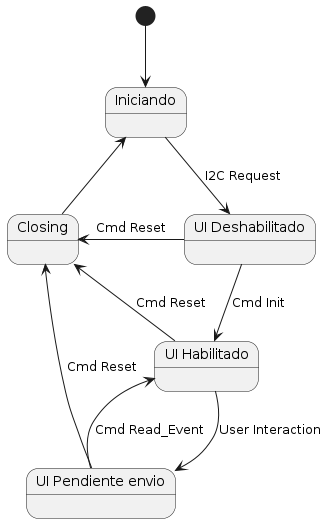
\includegraphics[scale=0.8]{images/states.png}
    \caption{Estados Dispositivos}
    \label{fig:deviceStates}
\end{figure}
En iniciando el dispositivo se acaba de iniciar (o de resetear) y esta a la espera de la primera request I2C.
En cuyo caso pasa a UI Deshabilitado, estado en el que el dispositivo respondera únicamente a peticiones I2C,
ignorando “todo” lo que haga el usuario.

Ante un comando de Iniciar, se pasa el estado UI Habilitado, en este estado se espera que el usuario realice
acciones (pulsar botón, mover palancas,…) y en cuanto se captura algun evento se pase a UI Pendiente de envio.
En este estado la línea INT debe estar baja. Cuando el máster envíe un comando de leer se vuelve a UI Habilitado
y se libera la linea INT.

Se espera que los eventos del usuario se gestionen en una Cola, por lo que UI Habilitado seria equivalente a
Cola Vacía  y UI Pendiente de envio Cola con Datos.

Una vez recivido el comando de reset el dispositivo se pasa a un estado de reseto donde puede hacer limpieza
de recursos antes de hacer un reset real. El proceso de limpieza debe terminar siempre y ejcutar una
interrupcion del procesador para hacer un reset.

Los dispositivos son libres de ampliar este diagrama de estados siempre y cuando ante el master respondan de
una manera coherente con este diagrama. Para ello se recomienda no ampliarlo y tener un segundo estado interno.

\subsection{Proceso de inicio}
El master a su vez ejecuta los siguientes pasos:
\begin{itemize}
    \item{} Lista los dispositivos I2C. (@, R, Stop), siguiendo los ejemplos “I2C scan”, el resultado es una lista
          de dispositivos (si podemos capturar el evento, el client bajara un pulso de su INT y registramos el pin INT)
    \item{} Para cada dispositivo ejecutara un proceso de identificación mandando varios comandos (ver seccion
          Identificacion) para comprobar que realmente es un dispositivo nuestro. En este
          paso detectaremos si hay algun conflicto (varios Dispositivos con la misma dirección I2C)
    \item{} Resolucion de conflictos (…)
    \item{} Inicializacion global (@=0)
\end{itemize}
A partir de este momento el master deberá estar mirando los pines de int y consultar el dispositivo cada vez que
este le baje a GND su linea de INT

\subsection{Identificación}
La identificación conlleva dos comandos, Obtener SN y Obtener Capacidades.

Las capacidades serán varios Bytes, siendo los primeros 6bits un identificador de tipo de panel (TFT, Botonera,….) 10 bits reservados para identificar hasta 10 protocolos básicos
(BTN, palancas, TFT,…) y luego bytes extra para incluir lista de protocolos soportados

Para cada protocolo se hará una consulta de capacidad a necesidad.

Luego estará el SN, que debe ser una cadena de bytes única para cualquier dipositivo, la idea es utilizar apis
de cada fabricante de microntrolador para usar el SN del dispositivo. Para que realmente sea único (por si
se da la casulidad de conflicto entre diferentes fabricantes) el primer byte sera un identificador de micro
(STM32, ATMEL, ESP32,…)
